% Part V (label part:3). Merged 2026-10-03 (author approval); input in main.tex after part5/p5_06_cmos.
% Carried from a private semiconductor analysis under the public/proprietary ruling of 2026-10-03: physics, method steps, design-family
% types and the caveats of the three published inputs. No class floors, no class exponents, no per-product readings beyond those already
% in Chapter ch:cmos. Numbers computed in docs/book/figscripts/fig_p3_platforms.py and MANIFEST.md of the delivery.
\chapter{Chips, generations and nodes on their own gauge}\label{ch:chipgen}

\section*{The place}
Every logically irreversible switching event is an irreversible information event, and conventional CMOS erases at almost every gate (Chapter~\ref{ch:cmos}). Physics establishes a minimum energy cost for every such
event, set by the operating temperature alone, with no dependence on transistor design, process node, foundry or manufacturer. It is not a
materials limit and not a lithography limit; it is IAM's Law at the transistor junction, $\kB T_j\ln2$ per bit (Chapter~\ref{ch:cmos}). The same floor applies wherever a bit is irreversibly set or erased, each substrate at its own temperature and with its own dominant
mechanism: a quantum gate whose error is later erased by correction, a switch driven by ionic conduction in a solid electrolyte, a spike in
a neuromorphic processor or a neural implant, a nucleotide coupled during DNA synthesis \interp. This
chapter reads a chip against that floor and against itself: what the three published numbers mean, how a chip's floor moves with its own
junction temperature, what a generation step on one definition says about the node, and how the reading applies to each design family. As
with qubits, the families are not ranked against each other \interp.

\section{The floor at the chip's own junction temperature}\label{sec:cg_floor}
The Landauer floor is $3.33\times10^{-21}$~J at 75\,$^\circ$C and $3.62\times10^{-21}$~J at 105\,$^\circ$C, 8.6\,\% higher \calc. The reading
$E_{\rm sw}=\mathrm{TDP}/(N_{\rm trans}f)$ carries no temperature, so the floor's position on a chip's gauge moves with the junction
temperature at which the chip actually runs: for the processor of Chapter~\ref{ch:cmos} ($E_{\rm sw}=1.92$--$1.98\times10^{-18}$~J) the floor
sits at 0.0017 at 75\,$^\circ$C and at 0.0018--0.0019 at 105\,$^\circ$C (Figure~\ref{fig:cg_floor_Tj}) \calc. The reliability floor of
Eq.~\eqref{eq:reliableswitch} moves in the same proportion. The real energy per switch also depends on temperature, through leakage, which
rises steeply, and through the voltage--frequency point; that dependence is a property of each design and is not part of the floor.

\begin{figure}[htbp]\centering
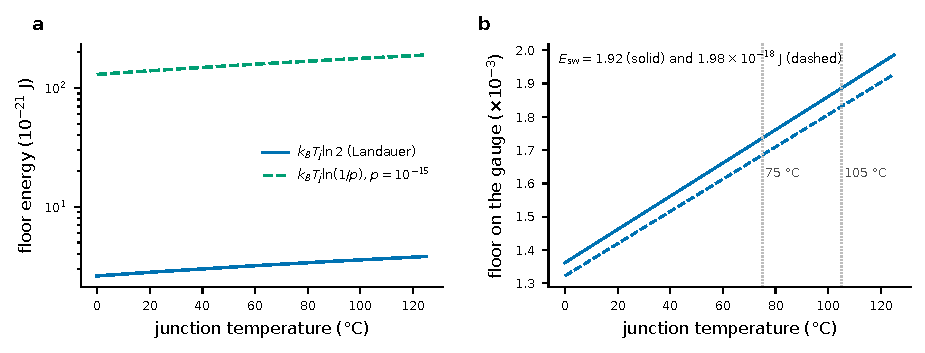
\includegraphics[width=\textwidth]{figures/part5/fig_p3_chip_floor_Tj.pdf}
\caption{(a) The Landauer floor $\kB T_j\ln2$ and the reliability floor $\kB T_j\ln(1/p)$ at $p=10^{-15}$ against junction temperature.
(b) Where the Landauer floor sits on the gauge of one chip read as built ($E_{\rm sw}=1.92$ and $1.98\times10^{-18}$~J, the two transistor
counts in circulation; Chapter~\ref{ch:cmos}). \calc}\label{fig:cg_floor_Tj}
\end{figure}

\section{Three published numbers, and what each one means}\label{sec:cg_inputs}
The chip gauge needs three numbers that appear on a maker's data sheet: a power, a transistor count and a clock. Each comes in more than one
kind, and the reading is only as definite as the definition used (Table~\ref{tab:cg_defs}).

\begin{table}[htbp]\centering\small
\caption{What the three inputs of the chip gauge can mean, and which way each choice moves the reading $E_{\rm sw}=\mathrm{TDP}/(Nf)$.}\label{tab:cg_defs}
\begin{tabularx}{\linewidth}{@{}>{\raggedright\arraybackslash}p{0.13\linewidth}>{\raggedright\arraybackslash}X>{\raggedright\arraybackslash}p{0.34\linewidth}@{}}\toprule
input & the kinds in use & effect on the reading \\\midrule
power & base (default) power; maximum turbo power; a board power for accelerators; for systems-on-chip whose makers publish none, third-party estimates & a maximum rating against a base rating differs by about a factor of two \\
transistors & total count including cache, graphics, neural and I/O blocks; die-level estimates where the maker publishes none & most of the count (SRAM) does not switch every cycle; the reading is a whole-chip average \\
clock & base clock; boost clock; all-core sustained clock & at fixed power a higher quoted clock lowers the reading with no change in energy per switch \\
hidden & activity factor; supply voltage and the point on the voltage--frequency curve; static power & dynamic energy scales as $CV^2$; static power is not switching \\\bottomrule
\end{tabularx}
\end{table}

Two worked cases show the size of the effect \calc. A generation pair in which the power figure changes from a maximum turbo rating of 253~W
to a base rating of 125~W reads a 70.7\,\% step; on one definition for both chips, with the newer chip also taken at a 253~W maximum turbo rating, the same pair reads $1-(1-0.707)\times253/125=40.7$\,\%.
One die at one board power quoted at 1.83 and at 1.98~GHz reads 7.6\,\% better at the higher clock (Chapter~\ref{ch:cmos}). A generation
comparison on the chip gauge is therefore made on one stated power, one stated clock and one stated count, or not at all.

\section{Generations and nodes}\label{sec:cg_nodes}
\paragraph{Two references for a node step.} Under constant-field scaling a node step that halves the area per transistor ($\kappa=\sqrt2$)
lowers the switching energy $CV^2$ by 64.6\,\%; at fixed voltage it lowers it by 29.3\,\% (Chapter~\ref{ch:cmos}, Figure~\ref{fig:switch_floors})
\derived. A measured step on one definition can be read against these two lines \interp. A step near 64.6\,\% per halving of area is what
voltage scaling delivers; a step near 29.3\,\% is what capacitance alone delivers once the voltage stops falling; a step below that says that
the energy per switch is being spent elsewhere, on leakage, on larger dies, on higher clocks; a step above 64.6\,\% says that something other
than the node changed, the design or the definition of an input.

\paragraph{The end of free scaling.} The breakdown was not caused by bad engineering at any particular company. Every manufacturer hit it at
roughly the same time because it was governed by the same underlying physics: transistors at small scales encounter leakage currents that
flow even when the transistor is off, and electric field strengths that prevent proportional voltage reduction. Power density stopped being
constant. The free ride ended. The 60~mV/decade subthreshold limit, $(\kB T/q)\ln10$, is the Boltzmann wall behind it (Chapter~\ref{ch:cmos})
\derived.

\paragraph{A step series that would cross the floor must end.} A chip that reads $R$ times its floor and improves by a constant fraction $s$
per generation reaches the floor after
\begin{equation}
 n_{\rm floor}=\frac{\ln R}{-\ln(1-s)}
 \label{eq:cg_nfloor}
\end{equation}
generations \derived. For $R=600$ that is 6.2 generations at the constant-field rate and 18.5 at the fixed-voltage rate \calc. The reading
cannot fall below the floor, so a series that would reach it in a few generations cannot continue at its present step; the step must shrink
before the floor is reached. When a chip's distance from the physical floor stops decreasing at the rate that node history predicts, a regime
change has occurred; the end of Dennard scaling is where the per-node steps of CMOS shrank \interp. Applying Eq.~\eqref{eq:cg_nfloor} to a
measured step requires the step on one definition (Section~\ref{sec:cg_inputs}); any fab can apply it to its own generation series.

\section{Design families}\label{sec:cg_families}
The reading applies to every family of CMOS logic in the same way, and each family carries its own caveats. Each is read against its own
as-built state and its own history on one definition \interp.
\begin{itemize}
\item \textbf{Single-die processors of the voltage-scaling era} (to about 2005). Supply voltage still fell with the node; per-node steps sat
near the constant-field line. Their transistor counts are small and mostly logic, so the whole-chip average is closest to the energy per
switching event \interp.
\item \textbf{Desktop and server processors after voltage scaling ended}, monolithic and chiplet. Power is quoted as a base, default or
maximum turbo figure; a chiplet part's count includes an I/O die whose transistors switch at a different rate and may sit on an older node.
The system-level reading is a weighted composite of dies at their own operating points \interp.
\item \textbf{Systems-on-chip with unified memory.} The count includes graphics, neural and memory-interface blocks; makers publish no power
figure, so the power is an estimate; the parts run at lower voltage and clock than desktop processors. Gaps between these and desktop
processors are confounded with operating point and die composition, and independent measurements find that the instruction set itself matters
little for energy~\cite{Blem2013} \conjecture\ for any architectural attribution.
\item \textbf{Graphics processors and accelerators.} GPU architecture makes a deliberate trade: it sacrifices per-transistor efficiency for
massive parallelism. The power is a board power, the clock a boost clock, much of the die is SRAM and memory interface, and some parts are two
dies in one package counted as one device. The reading measures energy per transistor per cycle, not throughput; for a workload the relevant
quantity is energy per operation \interp.
\end{itemize}

\section{Levers on the chip gauge}\label{sec:cg_levers}
When the node stops delivering, four levers remain: architecture, not node; chiplet specialization; the thermal operating regime; and
workload matching and scheduling. On the gauge only one of them moves the floor: the junction temperature, which moves $\kB T_j\ln2$ and the
reliability floor with it (Figure~\ref{fig:cg_floor_Tj}). The other three move the as-built reading \interp. Reversible logic is the one change
that would move a chip below the Landauer cost per operation, because only logically irreversible steps owe it~\cite{Bennett1973}
(Chapter~\ref{ch:cmos}).

\section{What a fab learns; what a referee would confirm}\label{sec:cg_use}
On one stated definition, the reading gives the energy per transistor per cycle, its distance from the floor at the chip's own junction
temperature, and where each generation step sits between the constant-field and fixed-voltage lines. To turn it into energy per switching
event a referee needs per-block power and activity from the design, the supply voltage and clock at the measured operating point, and the
junction temperature during the measurement; separating a node component from an architecture component needs the same data
(Chapter~\ref{ch:cmos}) \openprob.

\section{Status}
Derived: the floor's dependence on the chip's own junction temperature, the two node-step references and the step-series bound
Eq.~\eqref{eq:cg_nfloor} \derived. Calculated: the floor values, the floor positions and the worked definitional cases \calc. The readings of
generation steps against the two references, and the attribution of gaps between families, are \interp\ and \conjecture. Open: the
right-hand, full-surface mark of the chip gauge, and the per-block data that would turn the whole-chip average into an energy per switching
event \openprob.
